\documentclass[blue]{beamer}
\usetheme{Warsaw}
\usepackage{polski}
\usepackage[utf8]{inputenc}
\usepackage{amsmath}
\usepackage{amsfonts}
\usepackage{amssymb}
\usepackage{listings}
\usepackage{tikz}
\usepackage{url}
\author{matma6 (tech. Michał Gabor)}
\title{Programowanie logiczne w Prologu}
\date{26 marca 2013 r.}
\lstset{language=Prolog}
%to coś dodaje numery slajdów
\newcommand*\oldmacro{}%
\let\oldmacro\insertshorttitle%
\renewcommand*\insertshorttitle{%
  \oldmacro\hfill%
  \insertframenumber\,/\,\inserttotalframenumber}
%slajd tytułowy
\newcommand{\tytul}[1]{\begin{frame}\begin{center}\begin{Huge}#1\end{Huge}\end{center}\end{frame}}
\begin{document}
\begin{frame}
\titlepage
\end{frame}
\begin{frame}
\tableofcontents
\end{frame}
\section{Co to jest Prolog}
\tytul{Co to jest Prolog}
\subsection{Fakty}
\begin{frame}{Fakty}
\begin{itemize}
\item Francja, rok 1972
\item Alain Colmerauer i Philippe Roussel
\item Programowanie w logice (PROgrammation en LOGique)
\end{itemize}
\end{frame}
\subsection{Implementacje i instalacja}
\begin{frame}{Implementacje}
Istnieje wiele implementacji Prologu.
\begin{itemize}
\item SWI-Prolog
\item YAP
\item GNU Prolog
\item SICStus Prolog
\item Visual Prolog
\item ...
\end{itemize}
\end{frame}
\begin{frame}{SWI-Prolog}
Używam SWI-Prolog.

Cechy:
\begin{itemize}
\item LGPL/GPL
\item CLP
\item XPCE
\item Serwer WWW
\item Doskonała dokumentacja
\item ...
\end{itemize}
\end{frame}
\begin{frame}[fragile]{Instalacja}
\begin{description}
\item[Arch Linux] posiada SWI-Prolog w AURze (np.~\verb+yaourt -S swi-prolog+)
\item[Debian] ma SWI-Prolog w repozytorium (np.~\verb+sudo apt-get install swi-prolog+)
\item[MacOS X] paczka jest do pobrania ze strony \url{http://swi-prolog.org/}
\item[Windows] paczka jest do pobrania ze strony \url{http://swi-prolog.org/}
\end{description}

W GNU/Linuksie pojawia się wtedy polecenie \verb+swipl+.
\end{frame}
\subsection{Paradygmat logiczny}
\begin{frame}{Paradygmat logiczny}
\begin{description}
\item[Imperatywnie] wykonujemy instrukcje
\item[Funkcyjnie] obliczamy wartość funkcji
\item[Logicznie] pytamy o relacje
\end{description}
\end{frame}
\begin{frame}{Funkcja a relacja}
\begin{center}
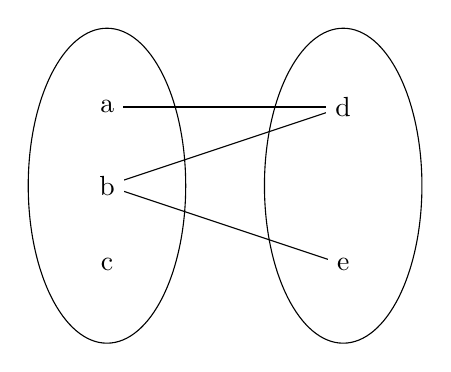
\begin{tikzpicture}
\draw (1, 3) -- (4, 3);
\draw (1, 2) -- (4, 3);
\draw (1, 2) -- (4, 1);
\draw (1, 2) ellipse (1 and 2);
\draw (1, 3) node [fill=white] {a};
\draw (1, 2) node [fill=white] {b};
\draw (1, 1) node [fill=white] {c};
\draw (4, 2) ellipse (1 and 2);
\draw (4, 3) node [fill=white] {d};
\draw (4, 1) node [fill=white] {e};
\end{tikzpicture}
\end{center}
\uncover<2->{
Relacja $\rho$ to nie funkcja:
\begin{description}
\item<3->[$\rho(a) = d$] ok...
\item<4->[$\rho(b) = ?$] dwie wartości
\item<5->[$\rho(c) = ?$] brak wartości
\end{description}}
\end{frame}
\begin{frame}[fragile]{W Prologu}
\begin{lstlisting}
ro(a, d).
ro(b, d).
ro(b, e).
\end{lstlisting}
\end{frame}
\begin{frame}[fragile]{Czas na przykład z życia - sinus :)}
\lstinputlisting{zrodla/lubi.pl}
\end{frame}
\section{Podstawy}
\tytul{Podstawy}
\subsection{Składnia}
\begin{frame}[fragile]{Komentarze, atomy i zmienne}
\begin{description}
\item[Komentarz] zaczyna się od \%.
\item[Atom] zaczyna się z małej litery.
\item[Zmienna] zaczyna się z dużej litery.\
\end{description}
\begin{lstlisting}
%atomy
jan
kot
pies

%Zmienne
Lista
X
N1
ODP
\end{lstlisting}
\end{frame}
\begin{frame}[fragile]{Źródło to nie REPL}
\begin{columns}
\begin{column}{.5\linewidth}
Źródło to baza faktów!

\lstinputlisting{zrodla/lubi.pl}
\end{column}
\begin{column}{.5\linewidth}
REPL służy do zadawania pytań!

\begin{lstlisting}
lubi(jan, koty).
lubi(jan, Co).
lubi(X, Y).
\end{lstlisting}
\end{column}
\end{columns}
Zarówno fakty, jak i pytania kończymy kropką.
\end{frame}
\subsection{Zmienne}
\begin{frame}[fragile]{Zmienne}
Prolog ma zmienne jednokrotnego przypisania:
\begin{lstlisting}
?- X = a.
X = a.

?- X = a, X = b.
false.

?- X = Y, X = 2.
X = Y, Y = 2.
\end{lstlisting}
\end{frame}
\begin{frame}[fragile]{Zmienne związane i wolne}
Jeśli zmienna ma wartość to jest związana (ang. grounded).

Zmienne mogące przyjąć różne wartości to zmienne wolne.
\begin{lstlisting}
?- X = 2, ground(X).
X = 2.

?- X = 2, ground(Y).
false.
\end{lstlisting}
\end{frame}
\begin{frame}[fragile]{Dopasowanie do wzorca}
Prolog wszędzie automatycznie dopasowuje się do wzorca.
\begin{lstlisting}
?- X = (a, b).
X = (a, b).

?- (X, Y) = (a, b).
X = a,
Y = b.

?- [_|T] = [a,b,c].
T = [b, c].
\end{lstlisting}
\_ to wieloznacznik

[X\textbar Y] to podział listy na głowę i ogon (OCamlowe H::T)
\end{frame}
\begin{frame}[fragile]{Zmienne a dane}
W Prologu zmienna może być częścią danej.
\begin{lstlisting}
?- (a, X) = (Y, b).
X = b,
Y = a.

?- length(X, 3).
X = [_G1106, _G1109, _G1112].

?- append([a, b, c], X, Y).
Y = [a, b, c | X].
\end{lstlisting}
\end{frame}
\subsection{Liczby i wyrażenia}
\begin{frame}[fragile]{2+2 to nie 4}
Prolog nie dokonuje ewaluacji automatycznie.

2+2 to wyrażenie

4 to liczba

Wyrażenie nie jest liczbą.

Żeby coś policzyć, używamy is.

\begin{lstlisting}
?- X = 2+2.
X = 2+2.

?- X is 2+2.
X = 4.
\end{lstlisting}
\end{frame}
\subsection{Listy i reguły}
\begin{frame}[fragile]{Długość listy}
\begin{columns}
\begin{column}{.5\linewidth}
\only<1>{
\begin{block}{Myśl logicznie!}
Długość listy pustej to 0.

Długość listy niepustej to długość ogona + 1.
\begin{center}inaczej\end{center}
Długość niepustej listy to N + 1 wtedy, gdy długość ogona to N.
\end{block}
}
\only<2>{
\begin{block}{Składnia reguły}
wniosek :- warunki.

Warunki oddzielamy przecinkiem (oraz)
\end{block}
}
\only<3-4>{
\begin{block}{Zagadka}
Co jest nie tak z tym kodem?

\uncover<4>{\alert<4>{Nie ma rekursji ogonowej.}}
\end{block}
}
\end{column}
\begin{column}{.5\linewidth}
\begin{lstlisting}
dl([], 0).

dl([_|T], N1) :-
    dl(T, N),
    N1 is N+1.
\end{lstlisting}
\end{column}
\end{columns}
\end{frame}
\begin{frame}[fragile]{Wersja optymalna z rekursją ogonową}
\lstinputlisting{zrodla/dlugosc.pl}
\end{frame}
\begin{frame}[fragile]{Czas na coś ciekawego}
\lstinputlisting{zrodla/polacz.pl}

Pytamy o relacje

A co Prolog na to?

\begin{lstlisting}
?- polacz(X, Y, [a,b,c]).
\end{lstlisting}
\end{frame}
\begin{frame}{Rozwidlanie}
W programach imperatywnych i funkcyjnych program ,,idzie'' jedną ścieżką.

W Prologu tworzone są równoległe ścieżki.

%\uncover<2>{Na przykład polacz/3.}
\end{frame}
\section{Ciekawe przykłady}
\tytul{Ciekawe przykłady}
\subsection{Listy różnicowe}
\tytul{Listy różnicowe}
\begin{frame}[fragile]{Definicja}
Lista różnicowa to lista z odjętym ogonem.
\begin{lstlisting}
[a, b, c, d] - [d]
[a, b, c | X] - X
\end{lstlisting}
\begin{enumerate}
\item Prolog nie ewaluuje, więc nie muszę definiować tego odejmowania
\item Mam daną listę [a, b, c], ale nie wiem, jaki ogon odejmę - zmienna częścią danej(!)
\item Te listy daje się (zwykle) łączyć w czasie stałym(!)
\end{enumerate}
\end{frame}
\begin{frame}[fragile]{Łączenie w czasie stałym}
Lista różnicowa to lista z odjętym ogonem.
\begin{lstlisting}
polacz(X-Y, Y-Z, X-Z).
\end{lstlisting}

Oto CAŁA implementacja.

Prolog cechuje bardzo zwięzły zapis.
\end{frame}
\subsection{Programy ,,samouczące się''}
\tytul{Programy ,,samouczące się''}
\begin{frame}{Ciąg Fibonacciego - z definicji}
\lstinputlisting{zrodla/fib1.pl}

\uncover<2>{Nieefektywne :(}
\end{frame}
\begin{frame}{Ciąg Fibonacciego - zapamiętajmy wynik}
\lstinputlisting{zrodla/fib.pl}
\end{frame}
\subsection{Zagadki}
\tytul{Zagadki}
\begin{frame}{Opis}
\textit{Zagadka pochodzi z ,,Jaki jest tytuł tej książki?'' autorstwa Raymonda Smullyana}

Wszyscy mieszkańcy pewnej wyspy są albo rycerzami (ludźmi, którzy nigdy nie kłamią) albo łotrami (ludźmi, którzy kłamią zawsze).

Wędrując po tej wyspie spotykamy trzech tubylców:

Zadaliśmy osobie A pytanie czy jest łotrem czy rycerzem ale ten odpowiedział niewyraźnie i nie zrozumieliśmy jego odpowiedzi.

Pytamy się osobę B co odpowiedział A. B odpowiada nam, że A powiedział o sobie, że jest łotrem.

Słysząc to C mówi: "Nie wierz B! To B jest łotrem!".

Kim są B i C?
\end{frame}
\begin{frame}{Kod}
\textit{Kod autorstwa dra Przemysława Kobylańskiego}
\lstinputlisting{zrodla/zagadka.pl}
\end{frame}
\begin{frame}[fragile]{Pytanie}
Pytamy się osobę B co odpowiedział A. B odpowiada nam, że A powiedział o sobie, że jest łotrem.

Słysząc to C mówi: "Nie wierz B! To B jest łotrem!".
\begin{lstlisting}
?- powiedzial(B, powiedzial(A, lotr(A))),
powiedzial(C, lotr(B)).

B = lotr,
C = rycerz.
\end{lstlisting}
\end{frame}
\subsection{Więzy}
\tytul{Więzy}
\begin{frame}{Czym są więzy}
Za pomocą więzów można zapisywać ograniczenia, np.
\begin{itemize}
\item A jest pomiędzy 0 i 9
\item A i B są różne
\end{itemize}

Przykłady podane za dokumentacją SWI-Prologu
\end{frame}
\begin{frame}{SEND + MORE = MONEY}
\begin{center}
\begin{Huge}
\begin{tabular}{cccccc}
 &  & S & E & N & D \\ 
+ &  & M & O & R & E \\ 
\hline 
 & M & O & N & E & Y \\ 
\end{tabular}
\end{Huge} 
\end{center}
\end{frame}
\begin{frame}[fragile]{SEND + MORE = MONEY}
Pytanie:
\begin{lstlisting}
?- puzzle(X + Y = Z), label(X).
\end{lstlisting}
\lstinputlisting{zrodla/money.pl}
\end{frame}
\begin{frame}{Sudoku}
\lstinputlisting{zrodla/sudoku.pl}
\end{frame}
\begin{frame}{Sudoku - konkretna zagadka}
\lstinputlisting{zrodla/sudoku-def.pl}
\end{frame}
\begin{frame}[fragile]{Sudoku - rozwiązanie}
\begin{lstlisting}
?- problem(1, Rows), sudoku(Rows),
   maplist(writeln, Rows).
[9, 8, 7, 6, 5, 4, 3, 2, 1]
[2, 4, 6, 1, 7, 3, 9, 8, 5]
[3, 5, 1, 9, 2, 8, 7, 4, 6]
[1, 2, 8, 5, 3, 7, 6, 9, 4]
[6, 3, 4, 8, 9, 2, 1, 5, 7]
[7, 9, 5, 4, 6, 1, 8, 3, 2]
[5, 1, 9, 2, 8, 6, 4, 7, 3]
[4, 7, 2, 3, 1, 9, 5, 6, 8]
[8, 6, 3, 7, 4, 5, 2, 1, 9]
Rows = [[9, 8, 7, 6, 5, 4, 3, 2|...], ... , [...|...]].
\end{lstlisting}
\end{frame}
\subsection{Funkcje anonimowe}
\tytul{Funkcje anonimowe}
\begin{frame}{Funkcje anonimowe}
\lstinputlisting{zrodla/fanon.pl}
\end{frame}
\section{Surgunt}
\tytul{Surgunt}
\begin{frame}[fragile]{Funkcje anonimowe}
\begin{lstlisting}
F = (X -> Y -> do(Z is X+Y) -> Z)

subst([2,3], F, R)

subst([1], F, Incr)
%Incr = (Y -> do(Z is 1+Y) -> Z)
\end{lstlisting}
\end{frame}
\begin{frame}{Funkcje anonimowe - kod 1/2}
\lstinputlisting{zrodla/surgunt/anonFun1.pl}
\end{frame}
\begin{frame}{Funkcje anonimowe - kod 2/2}
\lstinputlisting{zrodla/surgunt/anonFun2.pl}
\end{frame}
\begin{frame}[fragile]{Predykaty anonimowe}
\begin{lstlisting}
%zamiast pisac
length_(X, L) :- length(L, X).
?- length(Rows, 3), maplist(length_(3), Rows).

%mozemy napisac:
%anonPred(kod, interfejs, argument)
anonPred(length(L, 3), [L], List)

maplist(anonPred(length(L, 3), [L]), Rows)

%zatem dla kazdego wiersza:
anonPred(length(L, 3), [L], Row)
\end{lstlisting}
\end{frame}
\begin{frame}{Predykaty anonimowe - kod}
\lstinputlisting{zrodla/surgunt/anonPred.pl}
\end{frame}
\begin{frame}[fragile]{Składanie}
\begin{lstlisting}
%zamiast pisac
p1(Input, X1),
p2(Arg, X1, X2),
p3(X2, Output)

%piszemy
compose(Input, [p1, p2(Arg), p3], Output)
\end{lstlisting}
\end{frame}
\begin{frame}{Składanie - kod}
\lstinputlisting{zrodla/surgunt/compose.pl}
\end{frame}
\begin{frame}
\frametitle{Więcej informacji}
\begin{itemize}
\item E. Gatnar, K. Stąpor, \textit{Prolog, język sztucznej inteligencji}, PLJ, Warszawa 1991, ISBN: 83-85190-63-5
\item W. F. Clocksin, C. S. Mellish, \textit{Prolog, programowanie}, Helion, Gliwice 2003, ISBN: 83-7197-918-5
\item Jan Wielemaker, \textit{SWI-Prolog Reference Manual 6.2.6}, \url{http://www.swi-prolog.org/download/stable/doc/SWI-Prolog-6.2.6.pdf}
\end{itemize}
\end{frame}
\begin{frame}
\begin{center}
\begin{Huge}
Dziękuję za uwagę.

Czas na pytania.

matma6 (tech. Michał Gabor)

matma6.net

matma6@matma6.net

\end{Huge}
\end{center}
\end{frame}
\end{document}